% Pengaturan ukuran teks dan bentuk halaman dua sisi
\documentclass[10pt, twoside]{report}

% Pengaturan ukuran halaman dan margin
\usepackage[a5paper,top=25mm,left=25mm,right=20mm,bottom=25mm]{geometry}

% Pengaturan ukuran spasi
\usepackage[singlespacing]{setspace}

% Judul dokumen
\title{Buku Laporan Kerja Praktik ITC}
\author{Musk, Elon Reeve \and Kjellberg, Felix Arvid Ulf}

% Pengaturan format bahasa
\usepackage[indonesian]{babel}

% Pengaturan detail pada file PDF
\usepackage[pdfauthor={\@author},bookmarksnumbered,pdfborder={0 0 0}]{hyperref}

% Pengaturan jenis karakter
\usepackage[utf8]{inputenc}

% Package lainnya
\usepackage{etoolbox} % Mengubah fungsi default
\usepackage{enumitem} % Pembuatan list
\usepackage{lipsum} % Pembuatan template kalimat
\usepackage{graphicx} % Input gambar
\usepackage{longtable} % Pembuatan tabel
\usepackage[table,xcdraw]{xcolor} % Pewarnaan tabel
\usepackage{natbib} % Kutipan artikel
\usepackage{eso-pic} % Pembuatan background
\usepackage{changepage} % Pembuatan teks kolom
\usepackage{wrapfig} % Wrapping gambar

% Definisi untuk "Hati ini sengaja dikosongkan"
\def\kosong{
	\vspace*{\fill}
	\begin{center}\textit{Halaman ini sengaja dikosongkan}\end{center}
	\vfill
}
\patchcmd{\cleardoublepage}{\hbox{}}{\kosong}{}{}

% Pengaturan penomoran halaman
\usepackage{fancyhdr}
\fancyhf{}
\renewcommand{\headrulewidth}{0pt}
\pagestyle{fancy}
\fancyfoot[CE,CO]{\thepage}
\patchcmd{\chapter}{plain}{fancy}{}{}
\patchcmd{\chapter}{empty}{plain}{}{}

% Pengaturan format judul bab
\usepackage{titlesec}
\titleformat{\chapter}[display]{\bfseries\Large}{BAB \centering\Roman{chapter}}{0ex}{\vspace{0ex}\centering}[\vspace{2ex}]
\titleformat{\section}{\bfseries\large}{\MakeUppercase{\thesection}}{1ex}{}
\titleformat{\subsection}{\bfseries\large}{\MakeUppercase{\thesubsection}}{1ex}{}
\titleformat{\subsubsection}{\bfseries\large}{\MakeUppercase{\thesubsubsection}}{1ex}{}
\titlespacing*{\chapter}{0ex}{0ex}{0ex}
\titlespacing{\section}{0ex}{1ex}{1ex}
\titlespacing{\subsection}{0ex}{0.5ex}{0.5ex}
\titlespacing{\subsubsection}{0ex}{0ex}{0ex}

% Pengaturan persamaan
\newenvironment{conditions}
{\par\vspace{\abovedisplayskip}\noindent
	\tabularx{\columnwidth}{>{$}l<{$} @{${}={}$} >{\raggedright\arraybackslash}X}}
{\endtabularx\par\vspace{\belowdisplayskip}}

% Pengaturan format baris program
\usepackage{listings}
\definecolor{comment}{RGB}{0,128,0}
\definecolor{string}{RGB}{255,0,0}
\definecolor{keyword}{RGB}{0,0,255}
\lstdefinestyle{codestyle}{
	commentstyle=\color{comment},
	stringstyle=\color{string},
	keywordstyle=\color{keyword},
	basicstyle=\footnotesize\ttfamily,
	numbers=left,
	numberstyle=\tiny,
	numbersep=5pt,
	frame=lines,
	breaklines=true,
	prebreak=\raisebox{0ex}[0ex][0ex]{\ensuremath{\hookleftarrow}},
	showstringspaces=false,
	upquote=true,
	tabsize=2,
}
\lstset{style=codestyle}

% Isi keseluruhan dokumen
\begin{document}

  % Nomor halaman pembuka dimulai dari sini
  \pagenumbering{roman}

  % Sampul luar
  \AddToShipoutPictureBG*{
  \AtPageLowerLeft{
    % Ubah nilai berikut jika posisi horizontal background tidak sesuai
    \hspace{-3.5mm}

    % Ubah nilai berikut jika posisi vertikal background tidak sesuai
    \raisebox{0mm}{
      
\includegraphics[width=\paperwidth,height=\paperheight]{sampul/sampul-luar.png}
    }
  }
}

% Menyembunyikan nomor halaman
\thispagestyle{empty}

% Pengaturan margin untuk menyesuaikan konten sampul
\newgeometry{top=70mm,left=25mm,right=20mm,bottom=25mm}

\begin{flushleft}

  % Pengaturan jenis dan warna teks yang digunakan
  \sffamily\color{white}

  % Ubah penomoran buku berikut sesuai dengan yang ditentukan oleh departemen
  \noindent\textbf{KERJA PRAKTIK – EC184601}
  \vspace{4ex}

  % Ubah kalimat berikut sesuai dengan nama perusahaan tempat kerja praktik
  \noindent{\large \textbf{PT. ANEKA TUNA INDONESIA}} \\
  % Ubah tanggal berikut sesuai dengan waktu berlangsungnya kerja praktik
  \textbf{(06 Juli 2020 s/d 11 September 2020)}
  \vspace{6ex}

  % Ubah kalimat berikut sesuai dengan judul topik kerja praktik
  \noindent{\large \textbf{PEMBUATAN \emph{PROGRESSIVE WEB APP} UNTUK ADMINISTRASI LOADING BARANG BERBASIS \emph{NODE.JS}}}
  \vspace{6ex}

  \begin{adjustwidth}{-0.2cm}{}
    \begin{tabular}{lcp{0.7\linewidth}}
      % Ubah kalimat-kalimat berikut sesuai dengan nama dan NRP mahasiswa pertama
      \textbf{Muhammad Alfi Maulana Fikri} & & \textbf{NRP 0721 17 4000 0009} \\
      % Ubah kalimat-kalimat berikut sesuai dengan nama dan NRP mahasiswa kedua
      \textbf{Fairuz Fadilah Soemarsono} & & \textbf{NRP 0721 17 4000 0033} \\
    \end{tabular}
  \end{adjustwidth}
  \vspace{4ex}

  \noindent\textbf{Dosen Pembimbing} \\
  % Ubah kalimat berikut sesuai dengan nama dosen pembimbing
  \textbf{Arief Kurniawan, S.T., M.T.}
  \vspace{12ex}

  % Ubah kalimat berikut sesuai dengan nama departemen
  \noindent\textbf{DEPARTEMEN TEKNIK KOMPUTER} \\
  % Ubah kalimat berikut sesuai dengan nama fakultas
  \textbf{Fakultas Teknologi Elektro dan Informatika Cerdas} \\
  % Ubah kalimat berikut sesuai dengan nama universitas
  \textbf{Institut Teknologi Sepuluh Nopember} \\
  % Ubah kalimat berikut sesuai dengan tempat dan tahun pembuatan buku
  \textbf{Surabaya 2020}

\end{flushleft}

\restoregeometry
  \cleardoublepage

  % Sampul dalam
  \AddToShipoutPictureBG*{
  \AtPageLowerLeft{
    % Ubah nilai berikut jika posisi horizontal background tidak sesuai
    \hspace{-3.5mm}

    % Ubah nilai berikut jika posisi vertikal background tidak sesuai
    \raisebox{0mm}{
      
\includegraphics[width=\paperwidth,height=\paperheight]{sampul/sampul-dalam.png}
    }
  }
}

% Pengaturan margin untuk menyesuaikan konten sampul
\newgeometry{top=70mm,left=25mm,right=20mm,bottom=25mm}

\begin{flushleft}

  % Pengaturan jenis teks yang digunakan
  \sffamily

  % Ubah penomoran buku berikut sesuai dengan yang ditentukan oleh departemen
  \noindent\textbf{KERJA PRAKTIK – EC184601}
  \vspace{4ex}

  % Ubah kalimat berikut sesuai dengan nama perusahaan tempat kerja praktik
  \noindent{\large \textbf{PT. ANEKA TUNA INDONESIA}} \\
  % Ubah tanggal berikut sesuai dengan waktu berlangsungnya kerja praktik
  \textbf{(22 Juni 2020 s/d 25 Agustus 2020)}
  \vspace{6ex}

  % Ubah kalimat berikut sesuai dengan judul topik kerja praktik
  \noindent{\large \textbf{PEMBUATAN APLIKASI WEBSITE UNLOADING BASKET SECTION}}
  \vspace{6ex}

  \begin{adjustwidth}{-0.2cm}{}
    \begin{tabular}{lcp{0.7\linewidth}}
      % Ubah kalimat-kalimat berikut sesuai dengan nama dan NRP mahasiswa pertama
      \textbf{Muhammad Alfi Maulana Fikri} & & \textbf{NRP 0721 17 4000 0009} \\
      % Ubah kalimat-kalimat berikut sesuai dengan nama dan NRP mahasiswa kedua
      \textbf{Fairuz Fadilah Soemarsono} & & \textbf{NRP 0721 17 4000 0033} \\
    \end{tabular}
  \end{adjustwidth}
  \vspace{4ex}

  \noindent
  \textbf{Dosen Pembimbing} \\
  % Ubah kalimat berikut sesuai dengan nama dosen pembimbing
  \textbf{Arief Kurniawan, S.T., M.T.}
  \vspace{12ex}

  % Ubah kalimat berikut sesuai dengan nama departemen
  \noindent\textbf{DEPARTEMEN TEKNIK KOMPUTER} \\
  % Ubah kalimat berikut sesuai dengan nama fakultas
  \textbf{Fakultas Teknologi Elektro dan Informatika Cerdas} \\
  % Ubah kalimat berikut sesuai dengan nama universitas
  \textbf{Institut Teknologi Sepuluh Nopember} \\
  % Ubah kalimat berikut sesuai dengan tempat dan tahun pembuatan buku
  \textbf{Surabaya 2020}

\end{flushleft}

\restoregeometry
  \cleardoublepage

  % Lembar pengesahaan untuk departemen
  \begin{center}
  {\Large \textbf{LEMBAR PENGESAHAN}}
  \vspace{4ex}

  \addcontentsline{toc}{chapter}{LEMBAR PENGESAHAN (DEPARTEMEN)}

  % Ubah kalimat berikut sesuai dengan judul topik kerja praktik
  {\large \textbf{PEMBUATAN \emph{PROGRESSIVE WEB APP} UNTUK ADMINISTRASI LOADING BARANG BERBASIS \emph{NODE.JS}}} \\
  di \\
  PT. Aneka Tuna Indonesia
  \vspace{4ex}

  % Ubah kalimat berikut sesuai dengan kalimat pengesahan yang ditentukan oleh departemen
  Laporan Kerja Praktik ini disusun untuk memenuhi persyaratan akademik di Departemen Teknik Komputer FTEIC - ITS
  \vspace{2ex}

  % Ubah kalimat-kalimat berikut sesuai dengan tempat dan tanggal pengesahan
  Tempat Pengesahan di: Surabaya \\
  Tanggal: 1 Oktober 2020
  \vspace{8ex}

  Menyetujui, \\
  Dosen Pembimbing,
  \vspace{12ex}

  % Ubah kalimat-kalimat berikut sesuai dengan nama dan NIP dosen pembimbing
  \textbf{\underline{Arief Kurniawan, S.T., M.T.}} \\
  NIP. 19740907 200212 1 001
  \vspace{8ex}

  Mengetahui, \\
  % Ubah kalimat berikut sesuai dengan jabatan kepala departemen
  Kepala Departemen Teknik Komputer FTEIC - ITS,
  \vspace{12ex}

  % Ubah kalimat-kalimat berikut sesuai dengan nama dan NIP kepala departemen
  \textbf{\underline{Dr. Supeno Mardi Susiki Nugroho, S.T., M.T.}} \\
  NIP 19700313 199512 1 001

\end{center}
  \cleardoublepage

  % Lembar pengesahan untuk perusahaan
  \begin{center}
  {\Large \textbf{LEMBAR PENGESAHAN}}
  \vspace{4ex}

  \addcontentsline{toc}{chapter}{LEMBAR PENGESAHAN (PERUSAHAAN)}

  % Ubah kalimat berikut sesuai dengan judul topik kerja praktik
  {\large \textbf{PEMBUATAN APLIKASI WEBSITE UNLOADING BASKET SECTION}} \\
  di \\
  PT. Aneka Tuna Indonesia
  \vspace{4ex}

  % Ubah kalimat berikut sesuai dengan kalimat pengesahan yang ditentukan oleh departemen
  Laporan Kerja Praktik ini disusun untuk memenuhi persyaratan akademik di Departemen Teknik Komputer FTEIC - ITS
  \vspace{2ex}

  % Ubah kalimat-kalimat berikut sesuai dengan tempat dan tanggal pengesahan
  Tempat Pengesahan di: Surabaya \\
  Tanggal: 12 Oktober 2020
  \vspace{8ex}

  Mengetahui, \\
  Pembimbing Perusahaan
  \vspace{12ex}

  % Ubah kalimat berikut sesuai dengan nama pembimbing perusahaan
  \textbf{\underline{Jarot Kusumo Wibowo}}
  \vspace{8ex}

  Mengetahui, \\
  % Ubah kalimat berikut sesuai dengan jabatan kepala perusahaan
  Technology Manager PT. Aneka Tuna Indonesia
  \vspace{12ex}

  % Ubah kalimat berikut sesuai dengan nama kepala perusahaan.
  \textbf{\underline{Wie Sian Lie}}

\end{center}
  \cleardoublepage

  % Kata pengantar
  \begin{center}
  \Large\textbf{KATA PENGANTAR}
\end{center}
\vspace{2ex}

\addcontentsline{toc}{chapter}{KATA PENGANTAR}

% Pengaturan ukuran indentasi
\setlength{\parindent}{7ex}

% Ubah paragraf-paragraf berikut sesuai dengan yang ingin diisi pada kata pengantar

Puji syukur kami panjatkan kepada Allah SWT karena hanya dengan rahmat dan hidayah-Nya Penulis dapat melaksanakan kerja praktik dan menyelesaikan laporan kerja praktik di PT. Aneka Tuna Indonesia dengan topik “PEMBUATAN APLIKASI WEBSITE UNLOADING BASKET SECTION”.
Dalam pelakasanaan maupun penulisan laporan kerja praktik ini, Penulis mengucapkan terima kasih atas bantuan, arahan, dan motivasi yang diberikan baik secara langsung ataupun tidak langsung dari:
\vspace{0.5ex}

\begin{enumerate}[nolistsep]

  \item Bapak Arief Kurniawan, S.T., M.T. selaku Dosen Pembimbing di Departemen Teknik Komputer FTEIC - ITS, yang telah memberikan bimbingan kepada kami selama mengerjakan kerja praktik di perusahaan.
  \vspace{0.5ex}

  \item Bapak Jarot Kusumo Wibowo yang telah banyak memberikan arahan kepada kami.
  \vspace{0.5ex}

  \item Semua anggota PT. Aneka Tuna Indonesia yang telah memberikan ilmu-ilmu baru kepada kami serta berkenan untuk kami wawancarai maupun kami ajak berdiskusi.
  \vspace{0.5ex}

  \item Serta semua pihak yang tidak bisa disebutkan satu-persatu yang turut membantu dan memperlancar jalannya kerja praktik ini.
  \vspace{0.5ex}

\end{enumerate}
\vspace{0.5ex}

Penulis menyadari bahwa masih banyak kekurangan dalam perancangan dan pembuatan laporan Kerja Praktik ini.
Semoga buku laporan kerja praktik ini dapat memberikan manfaat bagi para pembaca, khususnya bagi penulis sendiri.
\vspace{2ex}

\begin{flushright}
  \begin{tabular}[b]{c}
    % Ubah kalimat berikut sesuai dengan tempat, bulan, dan tahun penulisan
    Surabaya, 12 Oktober 2020
    \\
    \\
    \\
    \\
    Penulis
  \end{tabular}
\end{flushright}

  \cleardoublepage

  % Daftar isi
  \renewcommand*\contentsname{DAFTAR ISI}
  \addcontentsline{toc}{chapter}{\contentsname}
  \titlespacing*{\chapter}{0pt}{0ex}{0ex}
  \tableofcontents
  \cleardoublepage

  % Daftar gambar
  \renewcommand*\listfigurename{DAFTAR GAMBAR}
  \addcontentsline{toc}{chapter}{\listfigurename}
  \titlespacing*{\chapter}{0pt}{0ex}{0ex}
  \listoffigures
  \cleardoublepage

  % Daftar tabel
  \renewcommand*\listtablename{DAFTAR TABEL}
  \addcontentsline{toc}{chapter}{\listtablename}
  \titlespacing*{\chapter}{0pt}{0ex}{0ex}
  \listoftables
  \cleardoublepage

  % Nomor halaman isi dimulai dari sini
  \pagenumbering{arabic}

  % Bab 1 pendahuluan
	% Ubah kalimat sesuai dengan judul dari bab ini
\chapter{PENDAHULUAN}
\vspace{4ex}

% Pengaturan ukuran indentasi
\setlength{\parindent}{7ex}

% Ubah konten-konten berikut sesuai dengan yang ingin diisi pada bab ini

\section{Latar Belakang}
\vspace{1ex}

Sebagai bentuk realisasi kebijaksanaan pemerintah dalam peningkatan mutu pendidikan perguruan tinggi dan untuk mendukung program link and match antara perguruan tinggi dengan dunia industri, maka diperlukan suatu bentuk kerja sama antara pihak perguruan tinggi dengan praktisi industri.
\vspace{0.5ex}

Salah satu bentuk kerja sama yang nyata adalah dengan pelaksanaan Kerja praktik seperti yang tercantum dalam kurikulum di perguruan tinggi, dalam hal ini Institut Teknologi Sepuluh Nopember Surabaya, di lingkungan perusahaan yang menerapkan teknologi yang sesuai dengan bidang studi mahasiswa.
Mata kuliah Kerja Praktik diharapkan dapat mendorong mahasiswa untuk mengenal kondisi di lapangan kerja dan untuk melihat keselarasan antara ilmu pengetahuan yang diperoleh di bangku kuliah dengan aplikasi praktis di dunia kerja.
\vspace{0.5ex}

PT. Aneka Tuna Indonesia sebagai salah satu perusahaan yang bergerak di bidang produksi ikan kaleng di Indonesia, diharapkan dapat menjembatani upaya-upaya perguruan tinggi dalam meningkatkan mutu pendidikannya melalui Kerja praktik sehingga membantu meningkatkan kualitas lulusan perguruan tinggi yang berdaya saing tinggi di dunia industri.
\vspace{0.5ex}

Dalam kerja praktik yang dilakukan, pekerjaan yang dilakukan adalah proses pembuatan aplikasi berbasis web untuk administrasi loading basket di PT. Aneka Tuna Indonesia.

\newpage

\section{Waktu dan Tempat Pelaksanaan}
\vspace{1ex}

Kerja praktik dilakukan secara Work From Home, dengan dua kali kunjungan di pabrik PT. Aneka Tuna Indonesia, yang beralamant di Jl. Randupitu - Gunung Gangsir No. 36, Asabri, Nogosari, Kec. Pandaan, Pasuruan, Jawa Timur 67156, dari tanggal 22 Juni 2020 sampai dengan 25 Agustus 2020.
\vspace{0.5ex}

\section{Tujuan}
\vspace{1ex}

Secara umum, tujuan dari kerja praktik ini adalah:
\vspace{0.5ex}

\begin{enumerate}[nolistsep]

  \item Menciptakan hubungan yang sinergis, jelas dan terarah antara dunia industri dan perguruan tinggi, dimana output perguruan tinggi merupakan sumber daya manusia dalam dunia industri.
  \vspace{0.5ex}

  \item Meningkatkan kepedulian dan partisipasi oleh dunia industri dalam memberikan kontribusi pada sistem pendidikan nasional.
  \vspace{0.5ex}

  \item Membuka wawasan mahasiswa agar dapat mengetahui dan memahami aplikasi ilmunya di dunia industri.
  \vspace{0.5ex}

  \item Sebagai sarana pembelajaran sosialisasi dalam lingkungan dunia kerja.
  \vspace{0.5ex}

  \item Mahasiswa dapat memahami dan mengetahui sistem kerja di dunia industri sekaligus mampu mengadakan pendekatan masalah yang ada.
  \vspace{0.5ex}

  \item Menumbuhkan dan menciptakan pola berpikir konstruktif yang lebih berwawasan bagi mahasiswa serta meningkatkan kemampuan praktik di bidang pengembangan aplikasi berbasis web dan mengaplikasikan langsung ilmu yang telah dipelajari di Departemen Teknik Komputer FTEIC - ITS.
  \vspace{0.5ex}

  \item Meningkatkan kedisiplinan, kemandirian, dan kepekaan mahasiswa melalui budaya kerja di dalam perusahaan.
  \vspace{0.5ex}

\end{enumerate}
\vspace{0.5ex}

Serta secara khusus, tujuan dari kerja praktik ini adalah:
\vspace{0.5ex}

\begin{enumerate}[nolistsep]

  \item Untuk memenuhi beban satuan kredit semester (SKS) yang harus ditempuh sebagai persyaratan akademis di Departemen Teknik Komputer FTEIC - ITS.
  \vspace{0.5ex}

  \item Mengembangkan pengetahuan, sikap, keterampilan dan kemampuan profesi melalui penerapan ilmu, latihan kerja dan pengamatan teknik yang diterapkan di PT. Aneka Tuna Indonesia.
  \vspace{0.5ex}

  \item Memperdalam pengetahuan mahasiswa dengan mengenal dan mempelajari secara langsung penerapan ilmu teknik komputer.
  \vspace{0.5ex}

  \item Mengembangkan hubungan baik antara pihak perguruan tinggi dengan PT. Aneka Tuna Indonesia.
  \vspace{0.5ex}

  \item Melakukan analisis dan memberikan rekomendasi dalam bentuk laporan kerja praktik kepada PT. Aneka Tuna Indonesia mengenai permasalahan yang dihadapi perusahaan.

\end{enumerate}
\vspace{0.5ex}

\section{Batasan Masalah}
\vspace{1ex}

Dalam penulisan laporan ini akan dibahas tentang pembuatan aplikasi berbasis web untuk administrasi loading basket di PT. Aneka Tuna Indonesia.
\vspace{0.5ex}

\section{Metodologi Pengumpulan Data}
\vspace{1ex}

Metodologi yang digunakan pada penyusunan laporan kerja ini adalah:
\vspace{0.5ex}

\begin{enumerate}[nolistsep]

  \item \textbf{Metode Eksperimen}
  \vspace{0.5ex}

  Penulis memperoleh data melalui percobaan langsung pada objek sehingga dapat mengamati pengaruh setiap komponen objek dan hubungan mereka disertai pencatatan tentang pengertian dan fungsi objek dengan singkat dan jelas.
  \vspace{0.5ex}

  \item \textbf{Studi Literatur}
  \vspace{0.5ex}

  Penulis mencatat atau memanfaatkan referensi berupa katalog, arsip-arsip, dan buku-buku. Referensi diperoleh dari perpustakaan dan dokumen perusahaan.
  \vspace{0.5ex}

  \item \textbf{Metode Diskusi}
  \vspace{0.5ex}

  Penulis mengumpulkan data melalui diskusi atau menanyakan secara langsung kepada pembimbing dan pegawai.
  Tujuannya untuk mendapatkan data-data secara langsung dan jelas.
  \vspace{0.5ex}

\end{enumerate}
\vspace{0.5ex}

\section{Sistematika Penulisan}
\vspace{1ex}

Dalam penulisan laporan kerja praktik ini, penulis membagi laporan dalam beberapa bab yang disusun dengan sistematika sebagai berikut:
\vspace{0.5ex}

\begin{enumerate}[nolistsep]

  \item \textbf{Bab I Pendahuluan}
  \vspace{0.5ex}

  Bab ini memaparkan mengenai garis besar kerja praktik yang meliputi latar belakang, waktu dan tempat pelaksanaan, tujuan kerja praktik, batasan masalah, metodologi pengumpulan data, serta sistematika penulisan laporan kerja praktik.
  \vspace{0.5ex}

  \item \textbf{Bab II Profil Perusahaan}
  \vspace{0.5ex}

  Bab ini berisi penjelasan mengenai profil PT. Aneka Tuna Indonesia yang meliputi sejarah, visi dan misi, dan struktur organisasi yang ada di perusahaan tersebut.
  \vspace{0.5ex}

  \item \textbf{Bab III Tinjauan Pustaka}
  \vspace{0.5ex}

  Bab ini berisi penjelasan tentang istilah-istilah atau teori-teori yang digunakan dalam pembuatan kerja praktik dan pustaka yang dipakai.
  \vspace{0.5ex}

  \item \textbf{Bab IV Desain dan Implementasi}
  \vspace{0.5ex}

  Bab ini berisi pemaparan mengenai kebutuhan untuk perancangan beserta implementasi dari sistem yang akan dibangun dan dikembangkan.
  \vspace{0.5ex}

  \item \textbf{Bab V Pengujian dan Evaluasi}
  \vspace{0.5ex}

  Bab ini berisi penjelasan tentang hasil pengujian sistem dan evaluasi yang dilakukan terhadap kinerja sistem secara menyeluruh.
  \vspace{0.5ex}

  \item \textbf{Bab VI Kesimpulan dan Saran}
  \vspace{0.5ex}

  Bab ini berisi kesimpulan dan saran dari proses selama pengerjaan kerja praktik di PT. Aneka Tuna Indonesia.
  \vspace{0.5ex}

\end{enumerate}
\vspace{0.5ex}

  \cleardoublepage

  % Bab 2 profil perusahaan
	% Ubah kalimat sesuai dengan judul dari bab ini
\chapter{PROFIL PERUSAHAAN}
\vspace{4ex}

% Pengaturan ukuran indentasi
\setlength{\parindent}{7ex}

% Ubah konten-konten berikut sesuai dengan yang ingin diisi pada bab ini

\section{Sejarah PT. Aneka Tuna Indonesia}
\vspace{1ex}

PT. Aneka Tuna Indonesia berdiri pada didirikan pada bulan Oktober 1991, sebagai perusahaan gabungan antara Itochu 
Corporation dan Hagoromo Foods Corporation, yang merupakan pemilik merek tuna terkemuka di Jepang, serta satu 
perusahaan asing lainnya. 
\vspace{0.5ex}

Terletak di daerah pegunungan dengan panorama eksotis di Provinsi Jawa Timur Indonesia, kami mulai beroperasi secara 
komersial pada bulan November 1992, mengkhususkan diri dalam produksi dan penjualan tuna kalengan. 
\vspace{0.5ex}

Itochu melakukan penjualan dan manajemen keseluruhan, sementara Hagoromo Foods bertanggung jawab atas produksi. 
Semua mitra secara aktif terlibat dalam peningkatan kualitas produk termasuk pengiriman teknisi dari Jepang dan 
pengiriman teknisi lokal ke Jepang untuk pelatihan.
\vspace{0.5ex}

\section{Visi dan Misi}
\vspace{1ex}

PT. Aneka Tuna Indonesia memiliki visi dan misi sebagai berikut:
\vspace{0.5ex}

\begin{enumerate}[nolistsep]

  \item \textbf{Visi PT. Aneka Tuna Indonesia}
  \vspace{0.5ex}

  Menjadi produsen tuna kaleng terkemuka di dunia.
  \vspace{0.5ex}

  \item \textbf{Misi PT. Aneka Tuna Indonesia}
  \vspace{0.5ex}

  \begin{enumerate}[nolistsep]

    \item Menjadikan semua stakeholder bagian penting dari perusahaan.
    \vspace{0.5ex}

    \item Menghasilkan produk yang berkualitas, sehat dan aman, serta ramah lingkungan.
    \vspace{0.5ex}

  \end{enumerate}
  \vspace{0.5ex}

\end{enumerate}
\vspace{0.5ex}

\section{Struktur Organisasi}
\vspace{1ex}

Struktur Organisasi dari PT. Aneka Tuna Indonesia adalah sebagai berikut.
\vspace{0.5ex}

% Contoh input gambar dengan format *.png
\begin{figure} [ht] \centering
  % Nama dari file gambar yang diinputkan
  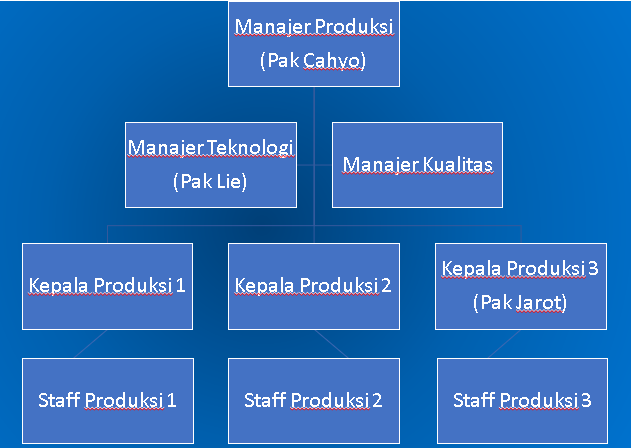
\includegraphics[scale=0.45]{gambar/hirarki-ATI.png}
  % Keterangan gambar yang diinputkan
  \caption{Struktur Organisasi PT. Aneka Tuna Indonesia}
  % Label referensi dari gambar yang diinputkan
	\label{fig:strukturOrganisasi}
\end{figure}

% Contoh penggunaan referensi dari gambar yang diinputkan
Seperti yang bisa dilihat pada gambar \ref{fig:strukturOrganisasi}, Pabrik ATI 2 (Pabrik Pandaan) yang terletak di 
Jl. Randupitu-Gunung Gangsir No.36, Asabri, Nogosari, Kec. Pandaan, Pasuruan, Jawa Timur dikepalai oleh seorang 
manajer produksi yaitu pak Cahyo Prabowo. Dengan dibantu oleh dua subordinat yaitu manajer kualitas dan manajer
teknologi yang dijabat oleh pak Wie Sian Lie. Produksi pada Pabrik ATI 2 dibagi menjadi tiga bagian, yaitu Produksi 1, 
Produksi 2, dan Produksi 3. Pada bagian Produksi 3 dikepalai oleh pak Jarot Wibowo Kusumo. Kepala Produksi 1, 2 , dan 3
membawahi staff yang sangat banyak (kurang lebih 3000 staff) yang terbagi menjadi beberapa tim dan juga shift kerja.
\vspace{0.5ex}

  \cleardoublepage

  % Bab 3 tunjauan pustaka
	% Ubah kalimat sesuai dengan judul dari bab ini
\chapter{TINJAUAN PUSTAKA}
\vspace{4ex}

% Pengaturan ukuran indentasi
\setlength{\parindent}{7ex}

% Ubah konten-konten berikut sesuai dengan yang ingin diisi pada bab ini

\section{\emph{Node.js}}
\vspace{1ex}

\emph{Node.js} merupakan \emph{runtime environment} untuk \emph{JavaScript} yang mampu membuat bahasa tersebut bisa dieksekusi diluar \emph{web browser}.
Umumnya \emph{Node.js} ini digunakan untuk membuat \emph{command line tools} dan untuk membuat program pada server.
Selain itu, \emph{Node.js} juga membantu pengembangan program berbahasa \emph{JavaScript} dengan memperkenalkan fitur modules dan packages, sehingga lebih banyak fitur yang bisa digunakan dalam pengembangan tanpa perlu menulis ulang kode program tersebut.
Saat ini, \emph{Node.js} sering kali digunakan sebagai alternatif dari \emph{PHP} untuk melakaukan \emph{server-side scripting}.
\vspace{0.5ex}

\section{\emph{Document-oriented Database}}
\vspace{1ex}

\emph{Document-oriented database} merupakan salah satu bentuk database dimana data yang ada disimpan dalam bentuk document yang menyerupai \emph{JSON}.
Database ini umumnya dikenal juga sebagai \emph{NoSql} (\emph{not only SQL}) karena berbeda dengan database \emph{SQL} pada umumnya yang disimpan dalam bentuk tabel terpisah yang saling memiliki relasi.
\vspace{0.5ex}

Beberapa keunggulan dari \emph{Document-oriented database} ini dibandingkan dengan database \emph{SQL} pada umumnya adalah sebagai berikut:
\vspace{0.5ex}

\begin{enumerate}[nolistsep]

  \item Memiliki model data yang intuitif, sehingga mudah dipahami dan dibuat oleh pengembang dan bisa langsung menyesuaikan objek yang ada pada baris program.
  \vspace{0.5ex}

  \item Skema yang fleksibel dan scalable, sehingga perubahan dari struktur data yang ada tidak akan banyak mempengaruhi data yang lain.
  Selain itu isi dari suatu data bisa berbeda dengan data yang lain tanpa adanya masalah.
  \vspace{0.5ex}

  \item Struktur database yang mennyerupai JSON mempermudah transfer data melalui internet karena umumnya data yang ada di internet dikirim dalam bentuk JSON.
  \vspace{0.5ex}

\end{enumerate}
\vspace{0.5ex}

\subsection{\emph{MongoDB}}
\vspace{1ex}

\emph{MongoDB} merupakan salah satu sistem yang menerapkan database dalam bentuk \emph{document-oriented}.
Database ini pertama kali diluncurkan 2009 oleh \emph{MongoDB Inc.} dan bisa diakses menggunakan berbagai macam bahasa seperti \emph{C++}, \emph{Go}, \emph{JavaScript}, dan \emph{Python}.
Untuk saat ini setidaknya terdapat dua versi dari \emph{MongoDB}, yang pertama merupakan versi \emph{Enterprise} yang ditujukan untuk kalangan bisnis dan perusahaan besar, dan yang kedua merupakan versi \emph{Community} yang bersifat \emph{open-source} dan bisa diakses secara gratis.
\vspace{0.5ex}

\subsection{\emph{Mongoose}}
\vspace{1ex}

\emph{Mongoose} merupakan tools yang digunakan pada program yang dibuat dengan \emph{Node.js} untuk mengakses database yang ada di \emph{MongoDB}.
Umumnya, \emph{Mongoose} digunakan untuk membuat schema atau model objek dari data yang akan disimpan di \emph{MongoDB}.
Selain itu tools ini juga bisa digunakan untuk menambahkan, mengubah, serta menghapus data yang ada di \emph{MongoDB} dengan query yang sudah ditentukan.
Dan juga sama seperti library di \emph{Node.js} lainnya yang bekerja secara \emph{asynchronous}, library ini bisa digunakan untuk mengakses database melalui fitur promises maupun callbacks yang ada di \emph{JavaScript}.
\vspace{0.5ex}

\section{\emph{Representational State Transfer API} (\emph{REST API})}
\vspace{1ex}

\emph{Representational state transfer} (\emph{REST}) merupakan salah satu gaya arsitektur untuk distributed hypermedia system yang pertama kali dicetuskan oleh Roy Fielding pada tahun 2000 \citep{rest}.
Kunci dari arsitektur \emph{REST} ini adalah adanya resource.
Setiap informasi yang bisa diberi nama adalah resource, mulai dari dokumen atau gambar, service, kumpulan data, dan lain sebagainya.
Selain itu pada \emph{REST} juga dikenal istilah resource methods yang berupa \emph{GET} yang digunakan untuk mengambil resource dari server, \emph{POST} yang digunakan untuk menambah resource baru, \emph{DELETE} yang digunakan utnuk menghapus resource yang ada, dan lain sebagainya.
\vspace{0.5ex}

Sama seperti gaya arsitektur yang lain, \emph{REST} juga mengenal adanya konstrain yang diperlukan agar suatu sistem dapat dikatakn sebagai \emph{RESTful}.
Konstrain tersebut adalah sebagai berikut:
\vspace{0.5ex}

\begin{enumerate}[nolistsep]

  \item Pemisahan antara client dan server sehingga bisa meningkatkan skalabilitas sistem pada berbagai macam platform.
  \vspace{0.5ex}

  \item Data request yang dikirim oleh client harus bersifat stateless, mengandung semua informasi yang dibutuhkan untuk memahami isi dari request tersebut.
  \vspace{0.5ex}

  \item Data yang direquest harus bisa digunakan kembali semisal client meminta hal tersebut, hal ini ditujukan untuk mengurangi request data yang sama berulang kali.
  \vspace{0.5ex}

  \item Interface yang uniform, sehingga bisa digunakan di berbagai macam platform.
  \vspace{0.5ex}

  \item Sistem yang bertingkat, sehingga pengembang hanya perlu fokus pada pengembangan di tingkat tertinggi yang diperlukan tanpa perlu ikut campur pada sistem yang ada di bawah.
  \vspace{0.5ex}

\end{enumerate}
\vspace{0.5ex}

\subsection{\emph{Express}}
\vspace{1ex}

\emph{Express}, dikenal juga sebagai \emph{Express.js}, merupakan \emph{framework back-end} untuk \emph{Node.js} yang dirilis sebagai \emph{free open-source} di bawah lisensi \emph{MIT}.
Framework ini dirancang untuk membangun aplikasi web dan API yang terinspirasi dari \emph{Sinatra}, \emph{framework back-end} berbahasa \emph{Ruby} yang relatif minimalis dan memiliki banyak fitur yang tersedia sebagai plugin.
Umumnya, framework ini digunakan bersamaan dengan beberapa komponene lain seperti \emph{Node.js}, \emph{MongoDB}, dan \emph{AngularJS} untuk membentuk \emph{MEAN} stack, sebuah alternatif dari \emph{XAMPP} yang dulunya banyak digunakan.
\vspace{0.5ex}

\newpage

\subsection{\emph{Axios}}
\vspace{1ex}

\emph{Axios} merupakan library pada \emph{JavaScript} yang digunakan sebagai \emph{HTTP client} pada web browser.
Library ini merupakan salah satu library yang bisa digunakan untuk mengakses \emph{REST API} secara \emph{asynchronous}.
Sama seperti prinsip pemrograman browser yang ada di \emph{JavaScript}, dengan sifat yang \emph{asynchronous} ini, sebuah proses request tidak akan mengganggu proses yang lain yang ada di client, sukses gagalnya dari proses tersebut bisa diatur menggunakan promises maupun callbacks yang ada pada \emph{JavaScript}.
\vspace{0.5ex}

\section{\emph{Progressive Web App} (\emph{PWA})}
\vspace{1ex}

\emph{Progressivw Web App} (\emph{PWA}) merupakan salah satu jenis aplikasi yang secara umum dipasang di website.
Model aplikasi ini kurang lebih sama dengan website pada umumnya dengan mengusung teknologi yang sama untuk pengembangannya seperti \emph{HTML}, \emph{CSS}, dan \emph{JavaScript} untuk bekerja pada platform manapun yang bisa bekerja dengan web browser.
\vspace{0.5ex}

Salah satu masalah dari aplikasi yang ada sekarang adalah, pada umumnya aplikasi native memiliki lebih banyak fitur seperti notifikasi, penyimpanan lokal, akses fitur yang ada di perangkat, dan lain sebagainya.
Namun aplikasi native ini hanya terbatas pada platform tertentu.
Di sisi lain terdapat website yang mampu dijangkau oleh semua platform secara general, baik desktop maupun mobile dengan berbagai macam distribusinya.
Namun website terkendala pada sifatnya yang strict dan tidak banyak fitur yang dimiliki dibandingkan dengan aplikasi native.
Di sini peran dari \emph{PWA} yang berada di tengah antara apliakasi native dan website, yang menjadikan sebuah aplikasi memiliki fitur yang lebih banyak mendekati native apps dan di sisi lain mudah diakses oleh berbagai macam platform yang mampu menjalankan web browser.
Dengan adanya \emph{PWA} ini, sebuah aplikasi dapat dengan mudah menjangkau berbagai kalangan dan di sisi lain memiliki fitur layaknya aplikasi umumnya seperti penyimpanan lokal, dan aplikasi.
\vspace{0.5ex}

\newpage

\subsection{\emph{Vue.js}}
\vspace{1ex}

\emph{Vue.js} merupakan salah satu framework front-end untuk \emph{Javascript} selain \emph{AngularJS} dan \emph{React} yang mampu digunakan untuk membuat antarmuka pada aplikasi yang interaktif dan responsif.
Secara umum \emph{Vue.js} mengubah baris program \emph{HTML} yang ada dalam bentuk template dan mengubahnya secara berkala ketika ada perubahan data yang berkaitan dengan baris program tersebut.
Pada \emph{Vue.js}, setiap bagian tatap muka dipisahkan menjadi berbagai macam components yang bisa digunakan secara berulang sehingga mengurangi penulisan program yang sama berulang-ulang.
Seperti \emph{Node.js}, \emph{Vue.js} juga mengenal packages (plugins) lain yang khusus dibuat untuk menambah fitur yang ada di \emph{Vue.js}.
Salah satu plugins tersebut adalah plugins \emph{PWA} yang digunakan untuk mengubah \emph{front-end} dari aplikasi yang dibuat agar bisa digunakan sebagai \emph{PWA}.
\vspace{0.5ex}

\subsection{\emph{Vuetify}}
\vspace{1ex}

\emph{Vuetify} merupakan library antarmuka yang digunakan untuk memperindah tampilan pada aplikasi yang dibuat menggunakan \emph{Vue.js}.
Fitur utama dari \emph{Vuetify} ini adalah untuk menyediakan berbagai macam components yang umumnya digunakan dalam pengembangan aplikasi seperti \emph{input field}, \emph{button}, \emph{navigation bar}, dan lain sebagainya.
Hal yang menarik dari \emph{Vuetify} ini adalah desain yang digunakan mengikuti prinsip \emph{Material Design} sehingga tampilan yang ada akan tampak standar sama seperti tampilan aplikasi yang umumnya ada saat ini, dengan menggunakan bentuk natural, warna yang tidak terlalu kontras, serta shading dan gradasi yang datar.
\vspace{0.5ex}

  \cleardoublepage

  % Bab 4 desain dan implementasi
	% Ubah kalimat sesuai dengan judul dari bab ini
\chapter{DESAIN DAN IMPLEMENTASI}
\vspace{4ex}

% Pengaturan ukuran indentasi
\setlength{\parindent}{7ex}

% Ubah konten-konten berikut sesuai dengan yang ingin diisi pada bab ini

\section{Deskripsi Sistem}
\vspace{1ex}

\lipsum[1]
\vspace{0.5ex}

\section{Spesifikasi Kasus Penggunaan}

\lipsum[2]
\vspace{0.5ex}

\section{Implementasi \emph{Database}}
\vspace{1ex}

\lipsum[3]
\vspace{0.5ex}

\section{Implementasi \emph{REST API}}
\vspace{1ex}

\lipsum[4]
\vspace{0.5ex}

\section{Implementasi Aplikasi}
\vspace{1ex}

Aplikasi diimplementasikan dengan \lipsum[2]
\vspace{0.5ex}

% Digunakan untuk page break
\newpage

% Contoh pembuatan code snippet
\begin{lstlisting}[
  language=C++,
  label={lst:helloWorld},
  caption={Hello World}
]
#include <iostream>

int main() {
    std::cout << "Hello World!";
    return 0;
}
\end{lstlisting}
\vspace{0.5ex}

% Contoh penggunaan referensi dari code snippet yang diinputkan
Seperti contoh pada baris program \ref{lst:helloWorld} dan \ref{lst:bilanganPrima}, \lipsum[3]
\vspace{0.5ex}

% Contoh input code snippet
\lstinputlisting[
  % Bahasa yang digunakan oleh code snippet
  language=Python,
  % Label referensi dari code snippet yang diinputkan
  label={lst:bilanganPrima},
  % Keterangan dari code snippet yang diinputkan
  caption={Perhitungan Bilangan Prima}
% Nama dari file code snippet yang diinputkan
]{program/prime-number.py}
\vspace{0.5ex}
  \cleardoublepage

  % Bab 5 pengujian dan evaluasi
	% Ubah kalimat sesuai dengan judul dari bab ini
\chapter{PENGUJIAN DAN EVALUASI}
\vspace{4ex}

% Pengaturan ukuran indentasi
\setlength{\parindent}{7ex}

% Ubah konten-konten berikut sesuai dengan yang ingin diisi pada bab ini

\section{Lingkungan Pengujian}
\vspace{1ex}

Pengujian yang kami lakukan menggunakan VPS (\emph{Virtual Private Server}) sebagai media yang digunakan untuk menjalankan sistem yang kami buat secara online.
Pada VPS tersebut, kami mempersiapkan beberapa hal yang diperlukan agar sistem bisa berjalan dengan semestinya.
Persiapan yang dijelaskan tersebut terdiri dari instalasi library dan framework yang dibutuhkan, instalasi dan konfigurasi database, konfigurasi DNS (\emph{Domain Name System}), konfigurasi service, dan lain sebagainya.
\vspace{0.5ex}

Setelah server sudah siap untuk digunakan, kami kemudian mempersiapkan dua jenis perangkat untuk menguji fungsionalitas dari sistem yang telah kami buat.
Pengujian tersebut akan dilakukan menggunakan sebuah perangkat desktop yang mengakses website secara langsung dan sebuah perangkat mobile yang mengakses server tersebut melalui PWA.
\vspace{0.5ex}

\section{Skenario Pengujian}
\vspace{1ex}

Pengujian yang kami lakukan akan mencakup keseluruhan aspek yang dimiliki oleh sistem yang telah kami buat.
Detail dari aspek-aspek tersebut adalah sebagai berikut:
\vspace{0.5ex}

\begin{enumerate}[nolistsep]

  \item Menguji sistem login dan pendaftaran akun baru.
  \vspace{0.5ex}

  \item Menguji penambahan, pengubahan, dan penghapusan data.
  \vspace{0.5ex}

  \item Menguji PWA pada perangkat mobile.
  \vspace{0.5ex}

  \item Menguji pengunduhan data dalam bentuk \emph{spreadsheet}.
  \vspace{0.5ex}

\end{enumerate}
\vspace{0.5ex}

\section{Tahapan Pengujian dan Evaluasi}
\vspace{1ex}

Pada bagian ini, kami akan membahas tahapan-tahapan pengujian yang kami lakukan beserta evaluasinya dengan memperhatikan aspek-aspek yang telah dijelaskan sebelumnya.
Untuk mempersingkat cakupan bahasan pada buku ini, pengujian tidak akan dilakukan pada keseluruhan fitur yang ada pada sistem yang kami buat, namun cukup beberapa fitur yang secara umum sudah mewakili aspek-aspek tersebut.
\vspace{0.5ex}

\subsection{Menguji Sistem Login dan Pendaftaran Akun Baru}
\vspace{1ex}

Pada pengujian ini, kami mencoba membuat akun baru pada sistem sesuai dengan yang ada pada gambar \ref{fig:mendaftarAkun}.
Akun baru yang dibuat ini nantinya akan digunakan oleh pihak karyawan yang ditugaskan untuk melakukan pencatatan administrasi loading barang agar bisa mengakses fungsionalitas pada sistem yang dibuat.
\vspace{0.5ex}

\begin{figure} [ht!] \centering
  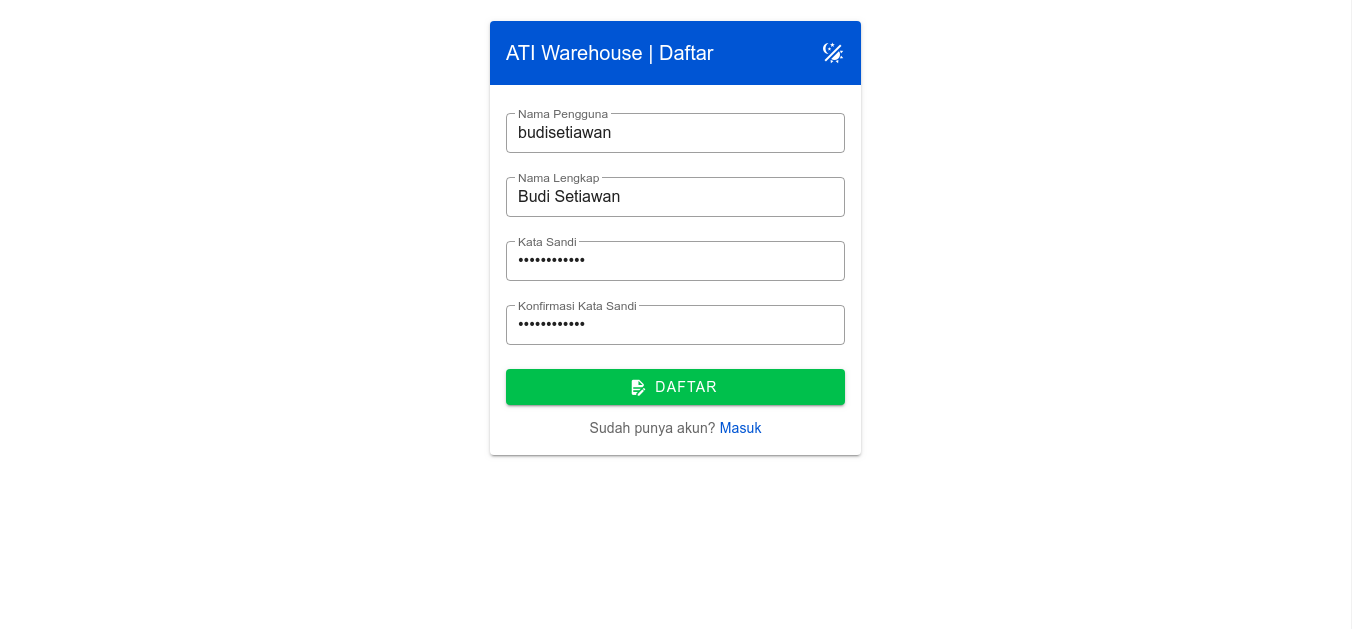
\includegraphics[width=0.95\textwidth]{gambar/mendaftar-akun.png}
  \caption{Tampilan Halaman Pendaftaran Akun Baru}
	\label{fig:mendaftarAkun}
\end{figure}

Pada sistem yang kami buat, sebelum bisa login, akun baru harus diverifikasi terlebih dahulu oleh admin untuk menghindari akses dari akun yang tidak diinginkan.
Verifikasi sendiri bisa dilakukan pada halaman daftar pengguna menggunakan akun admin seperti yang terlihat pada gambar \ref{fig:daftarPengguna}.
\vspace{0.5ex}

\begin{figure} [ht!] \centering
  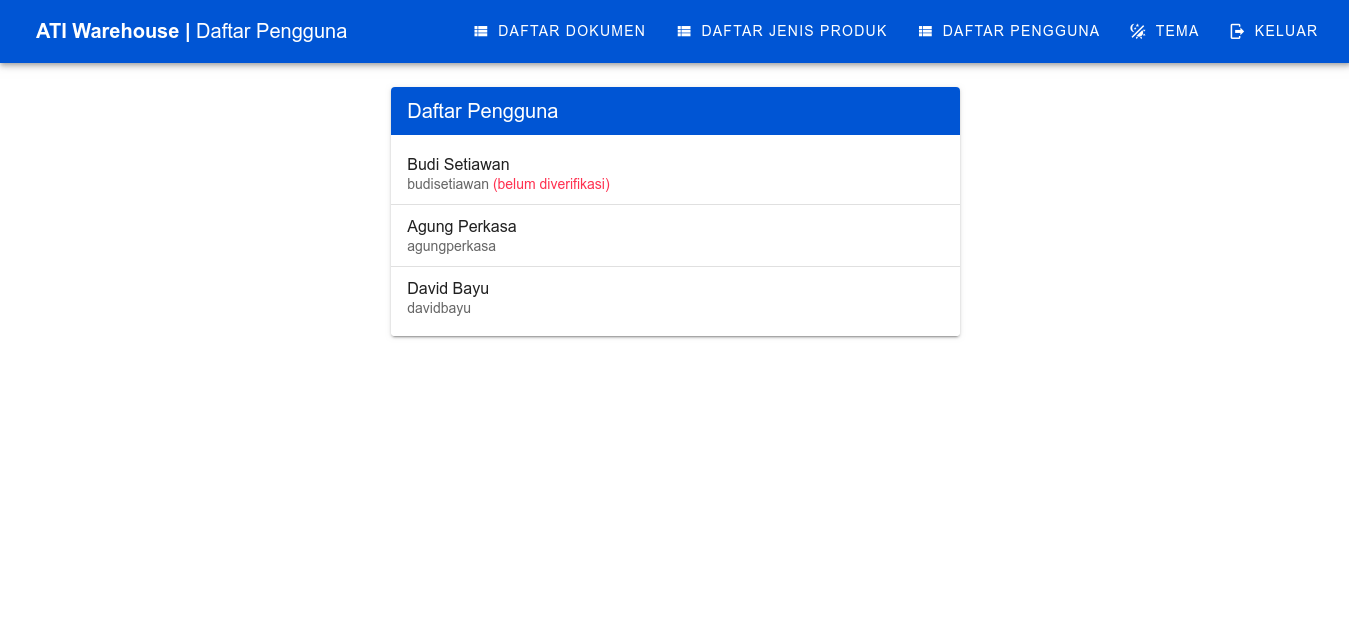
\includegraphics[width=0.95\textwidth]{gambar/daftar-pengguna.png}
  \caption{Tampilan Halaman Daftar Pengguna}
	\label{fig:daftarPengguna}
\end{figure}

Pengujian kemudian dilanjutkan dengan melakukan login menggunakan akun yang sudah diverifikasi sebelumnya seperti yang terlihat pada gambar \ref{fig:loginAkun}.
Setelah login berhasil, tampilan akan berpindah ke halaman utama yang berisi data dari keseluruhan administrasi loading barang.
\vspace{0.5ex}

\begin{figure} [ht!] \centering
  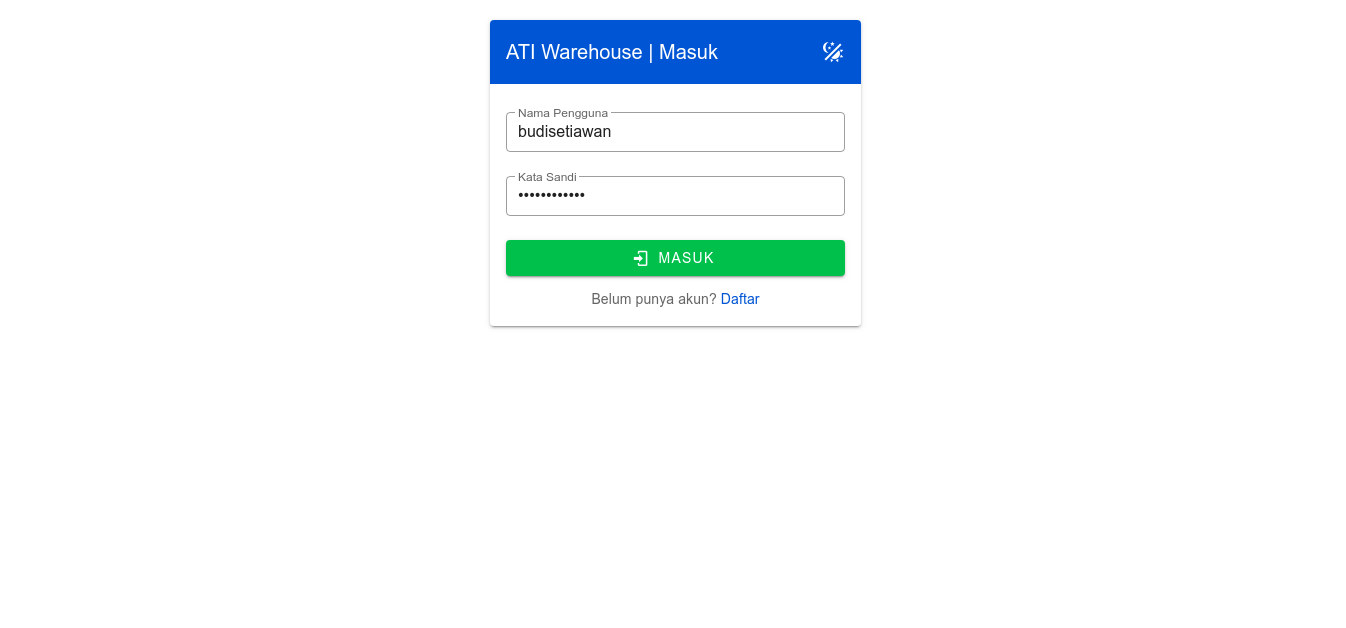
\includegraphics[width=0.95\textwidth]{gambar/login-akun.png}
  \caption{Tampilan Halaman Login Akun}
	\label{fig:loginAkun}
\end{figure}

Dari pengujian yang telah dilakukan tersebut dapat disimpulkan bahwa sistem yang telah kami buat bisa digunakan untuk melakukan login serta registrasi untuk pembuatan akun baru.
Dengan ini, nantinya pengguna yang membutuhkan akses terhadap data administrasi loading barang bisa membuat akun baru yang kemudian dapat diverifikasi oleh admin agar bisa mengakses data tersebut.
\vspace{0.5ex}

\subsection{Menguji Penambahan, Pengubahan, dan Penghapusan Data}
\vspace{1ex}

Pada pengujian ini, kami mencoba melakukan penambahan data palet sesuai dengan tabel \ref{tb:dataPalet}.
Penambahan data palet ini dilakukan pada halaman detail dokumen dengan mengklik tombol tambah data palet.
Setelah tombol diklik, maka akan muncul jendela baru seperti yang terlihat pada gambar \ref{fig:tambahPalet}.
\vspace{0.5ex}

\begin{longtable}{|l|l|l|l|l|}
	\caption{Data Palet}
	\label{tb:dataPalet}\\
  \hline
  \rowcolor[HTML]{C0C0C0}
  \textbf{Mulai} & \textbf{Selesai} & \textbf{Palet} & \textbf{Basket} & \textbf{Jumlah Layer} \\ \hline
	13:03 & 13:34 & 1 & 1, 2, 3 & 18 \\ \hline
	13:34 & 13:49 & 2 & 3, 4, 5 & 18 \\ \hline
	13:49 & 14:05 & 3 & 5, 6, 7 & 18 \\ \hline
	14:05 & 14:26 & 4 & 7, 8, 9 & 18 \\ \hline
	14:26 & 14:35 & 5 & 9, 10, 11, 12 & 18 \\ \hline
	14:35 & 14:50 & 6 & 12, 13, 14 & 18 \\ \hline
\end{longtable}

\begin{figure} [ht!] \centering
  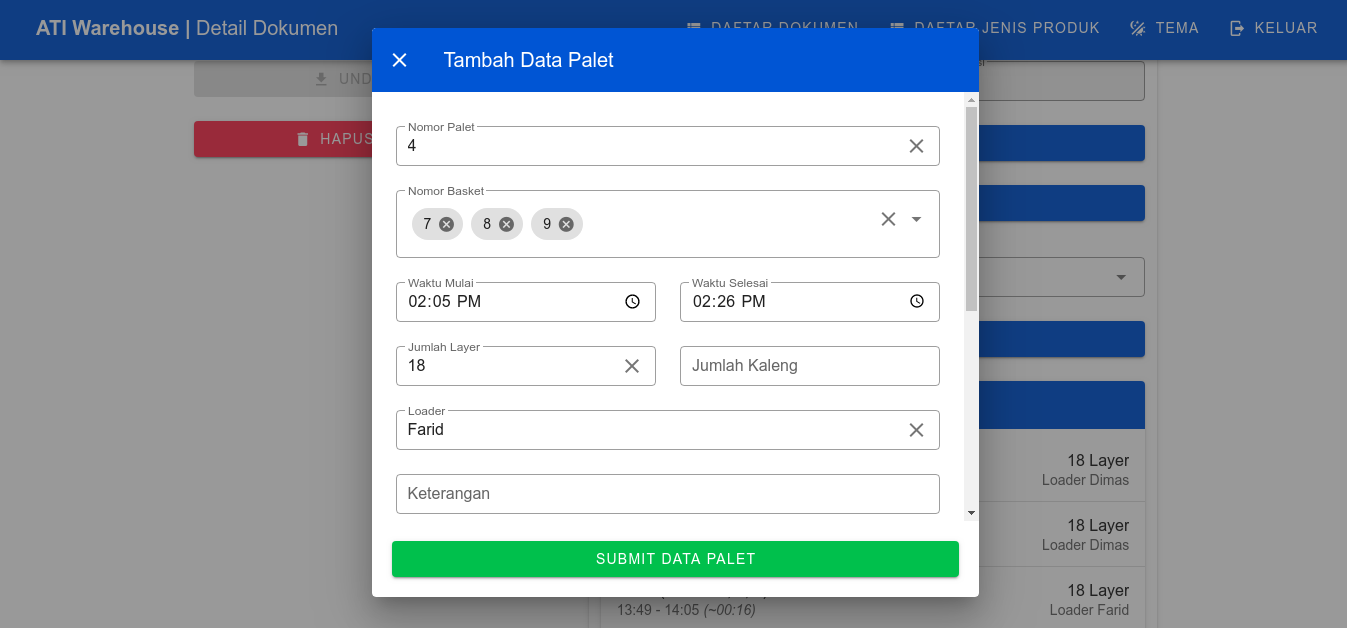
\includegraphics[width=0.95\textwidth]{gambar/tambah-palet.png}
  \caption{Tampilan Jendela Tambah Data Palet}
	\label{fig:tambahPalet}
\end{figure}

Pengujian kemudian dilanjutkan dengan mengubah jumlah layer pada palet nomor 5 menjadi sebanyak 15.
Pengubahan data palet ini dilakukan pada halaman detail palet seperti yang terlihat pada gambar \ref{fig:ubahPalet}.
\vspace{0.5ex}

\begin{figure} [ht!] \centering
  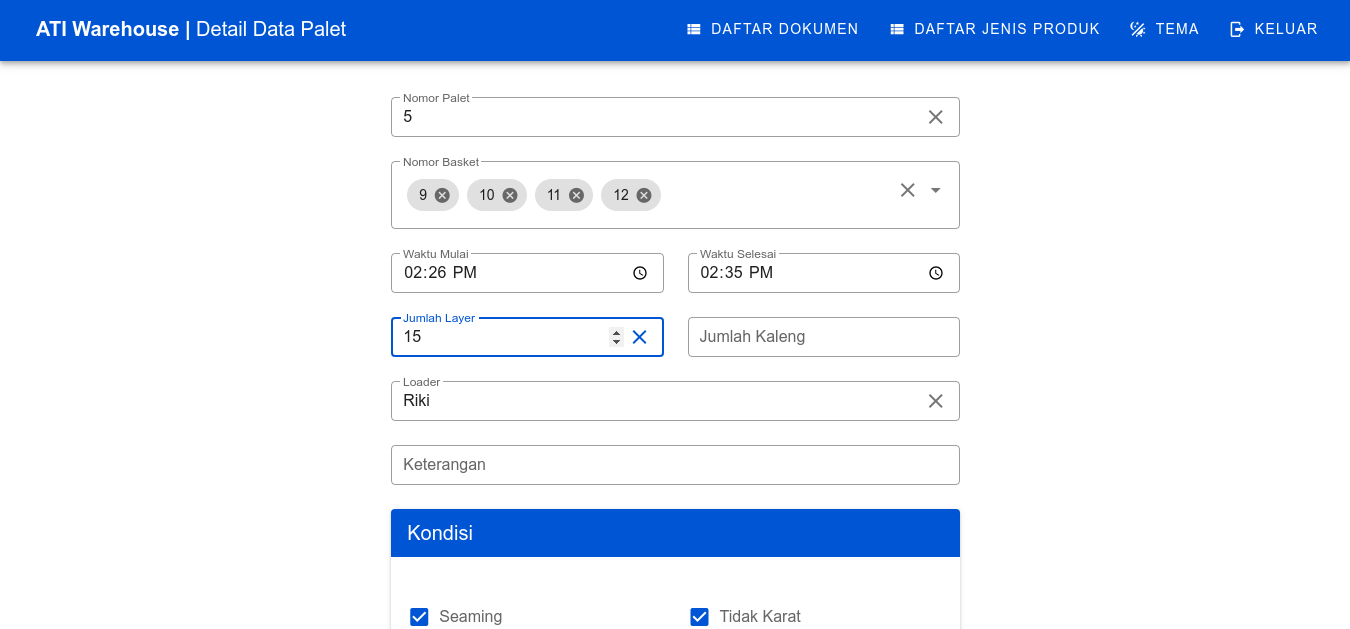
\includegraphics[width=0.95\textwidth]{gambar/ubah-palet.png}
  \caption{Tampilan Halaman Detail Palet}
	\label{fig:ubahPalet}
\end{figure}

Terakhir, pengujian kemudian dilanjutkan dengan menghapus data pada palet nomor 6.
Penghapusan data palet ini juga dilakukan pada halaman detail palet seperti pada percobaan sebelumnya dengan menekan tombol hapus data palet.
Hasil akhir dari percobaan ini adalah kumpulan data palet seperti yang terlihat pada gambar \ref{fig:daftarPalet}.
\vspace{0.5ex}

\begin{figure} [ht!] \centering
  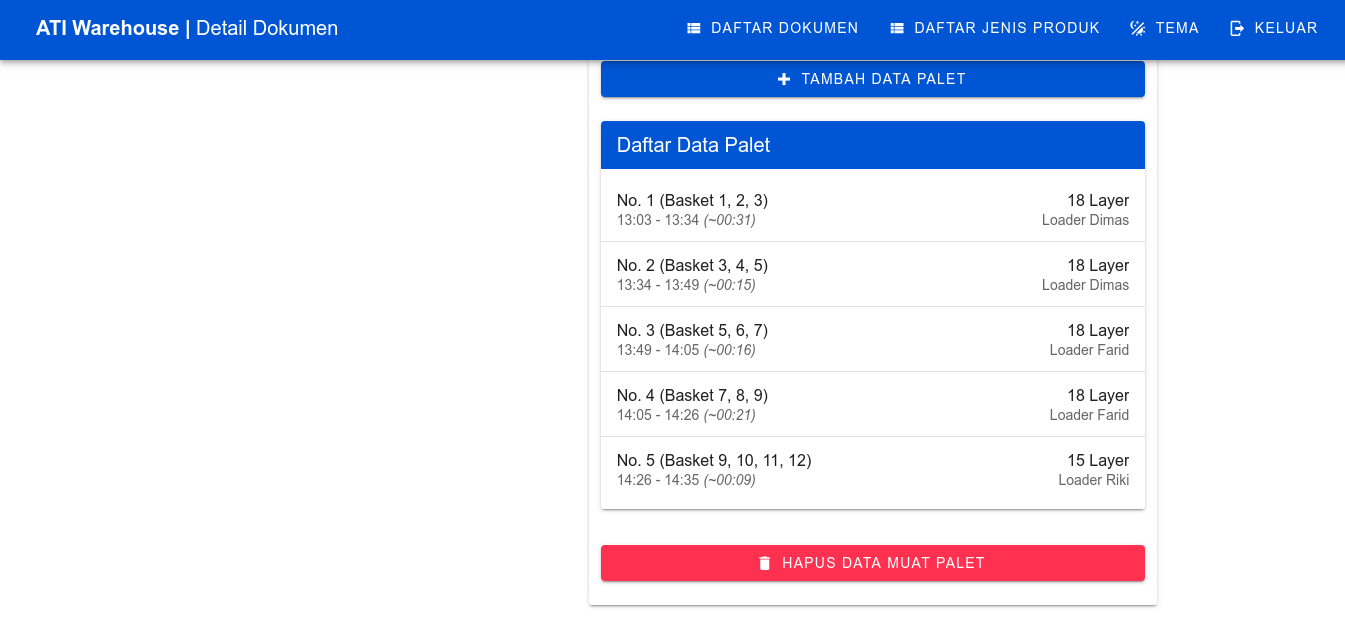
\includegraphics[width=0.95\textwidth]{gambar/daftar-palet.png}
  \caption{Tampilan Daftar Palet}
	\label{fig:daftarPalet}
\end{figure}

Dari pengujian yang telah dilakukan tersebut, dapat disimpulkan bahwa sistem yang telah kami buat bisa digunakan untuk melakukan penambahan, pengubahan, serta penghapusan data sesuai dengan struktur data yang telah ditentukan oleh sistem.
Dengan ini, nantinya sistem yang kami buat bisa digunakan untuk menampung serta menampilkan data administrasi loading barang, menggantikan metode sebelumnya yang masih berbasis kertas.
\vspace{0.5ex}

\subsection{Menguji PWA Pada Perangkat Mobile}
\vspace{1ex}

Pada pengujian kali ini, kami mencoba menguji penggunaan PWA dari system yang telah kita buat pada perangkat mobile.
Pemasangan PWA sendiri bisa dilakukan dengan cara mengakses website dari sistem yang telah kita buat pada perangkat mobile.
Pada website yang mendukung fitur PWA, umumnya browser akan menawarkan penambahan website tersebut sebagai aplikasi pada perangkat mobile seperti yang terlihat pada gambar \ref{fig:pasangPwa}.
\vspace{0.5ex}

\begin{figure} [ht!] \centering
  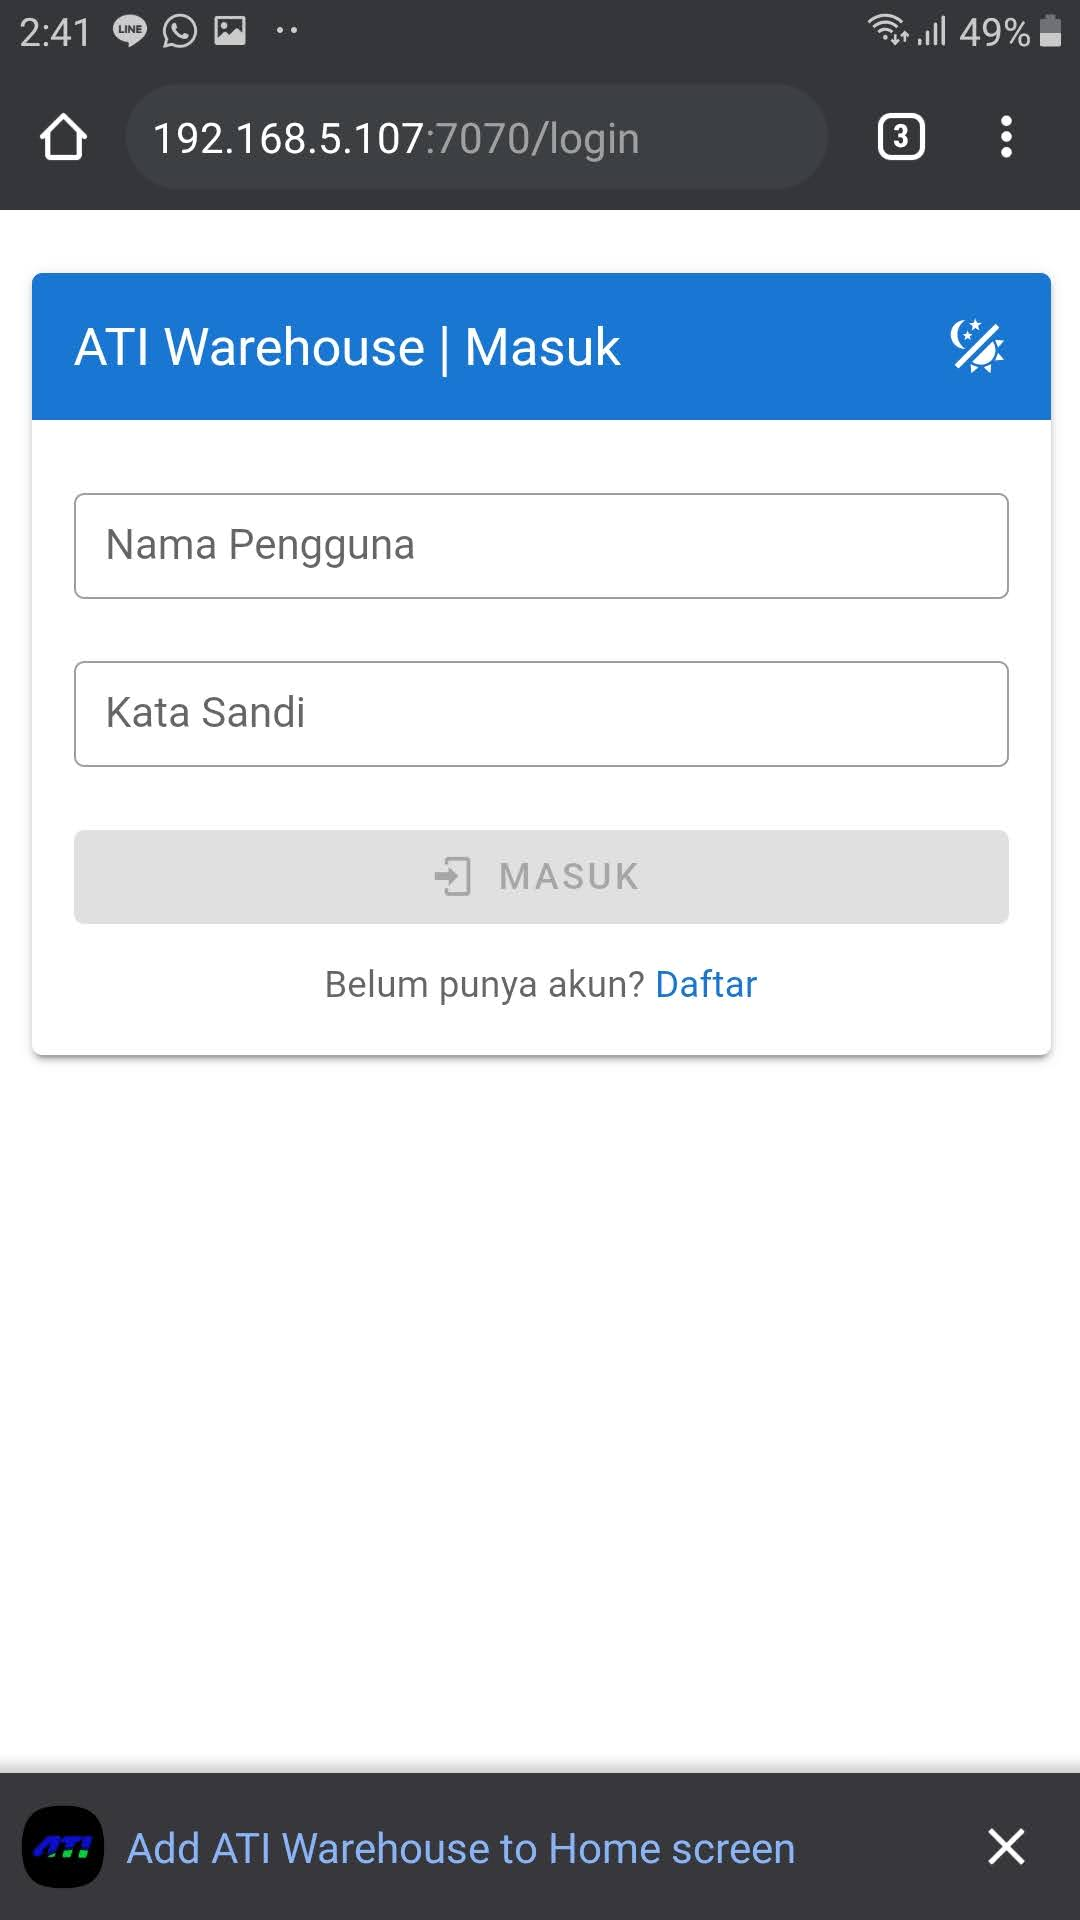
\includegraphics[width=0.45\textwidth]{gambar/pasang-pwa.jpg}
  \caption{Tawaran Penambahan Website Sebagai PWA}
	\label{fig:pasangPwa}
\end{figure}

Setelah terpasang, sistem yang kami buat akan tampak pada daftar aplikasi yang ada di perangkat mobile selayaknya aplikasi pada umumnya.
Selain itu, PWA yang telah kita pasang nantinya bisa berfungsi selayaknya sistem yang juga terpasang pada website seperti terlihat pada gambar \ref{fig:tampilanPwa}.
Dengan ini, alih-alih mengakses website untuk menggunakan sistem yang telah kami buat,  pengguna juga bisa memasang langsung sistem tersebut pada perangkat mereka, sehingga mempermudah akses dari sistem administrasi loading barang ini.

\begin{figure} [ht!] \centering
  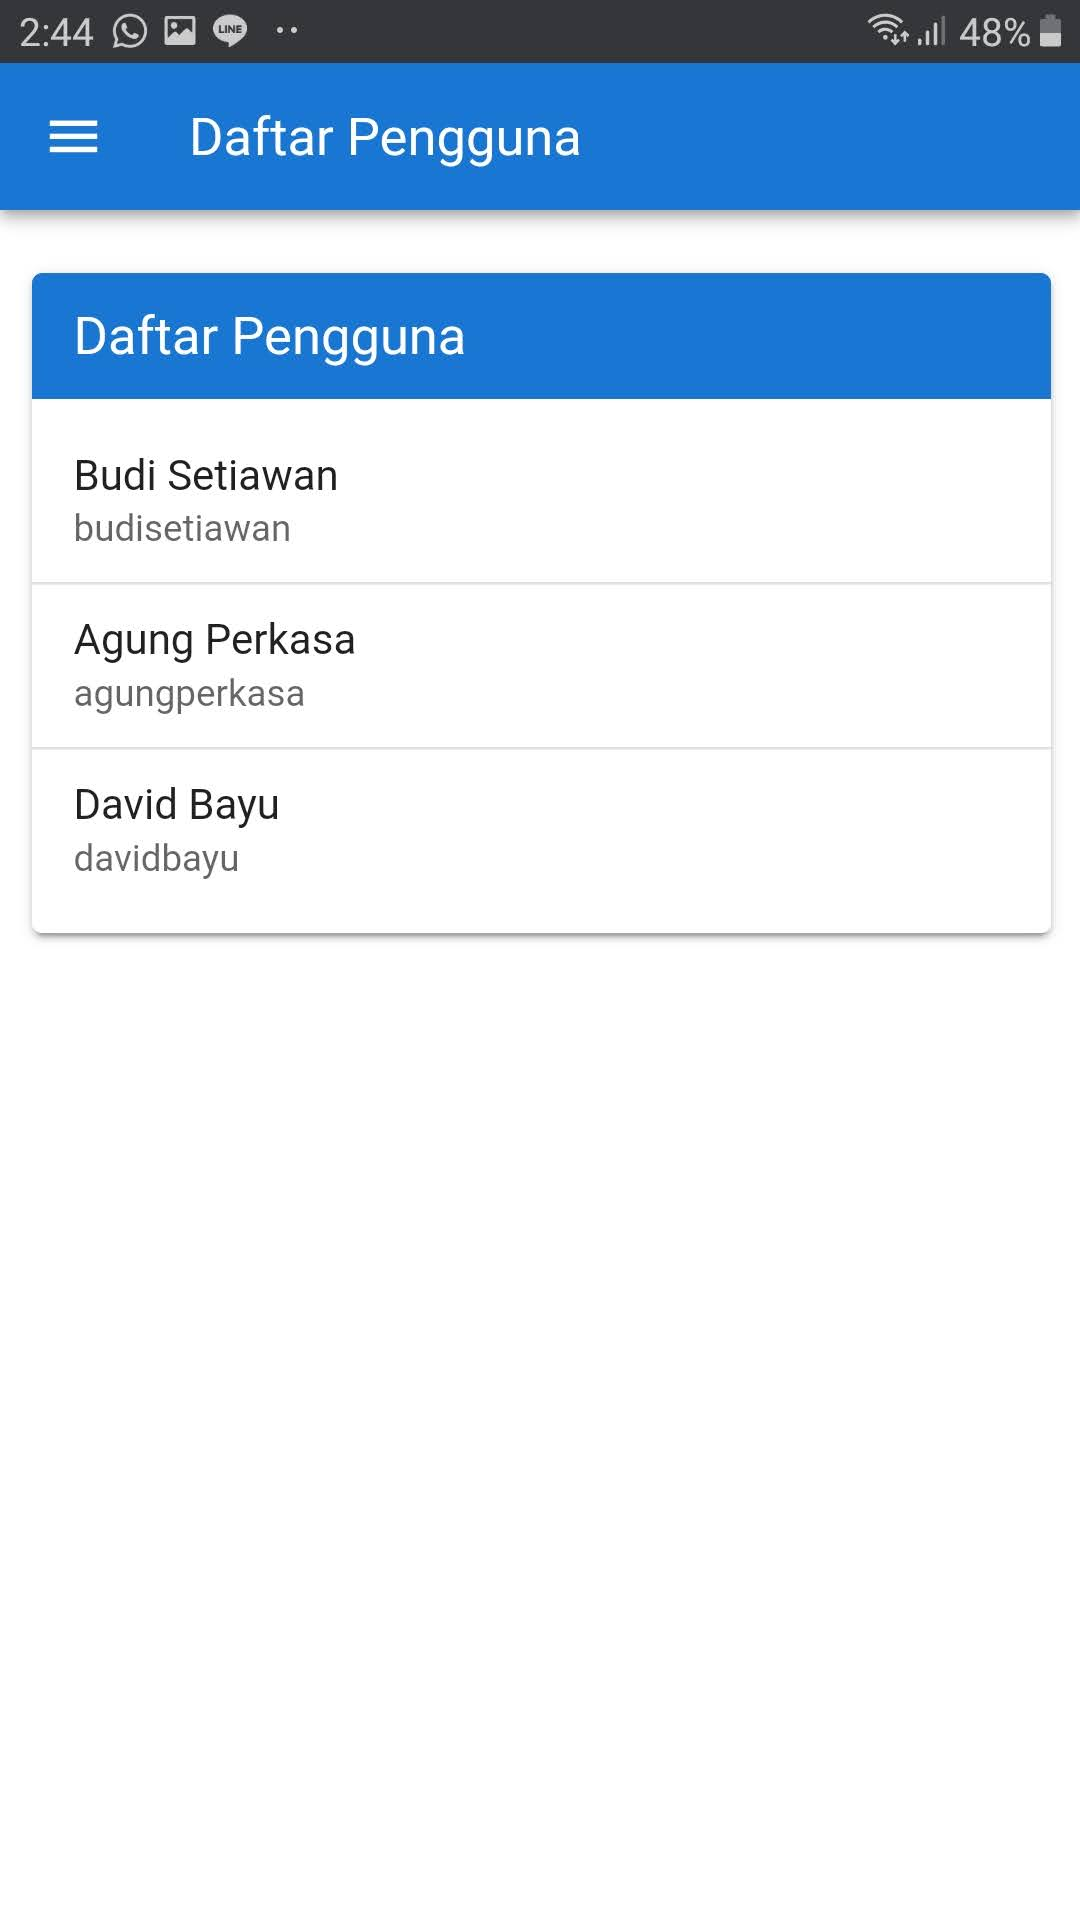
\includegraphics[width=0.45\textwidth]{gambar/tampilan-pwa-1.jpg}
  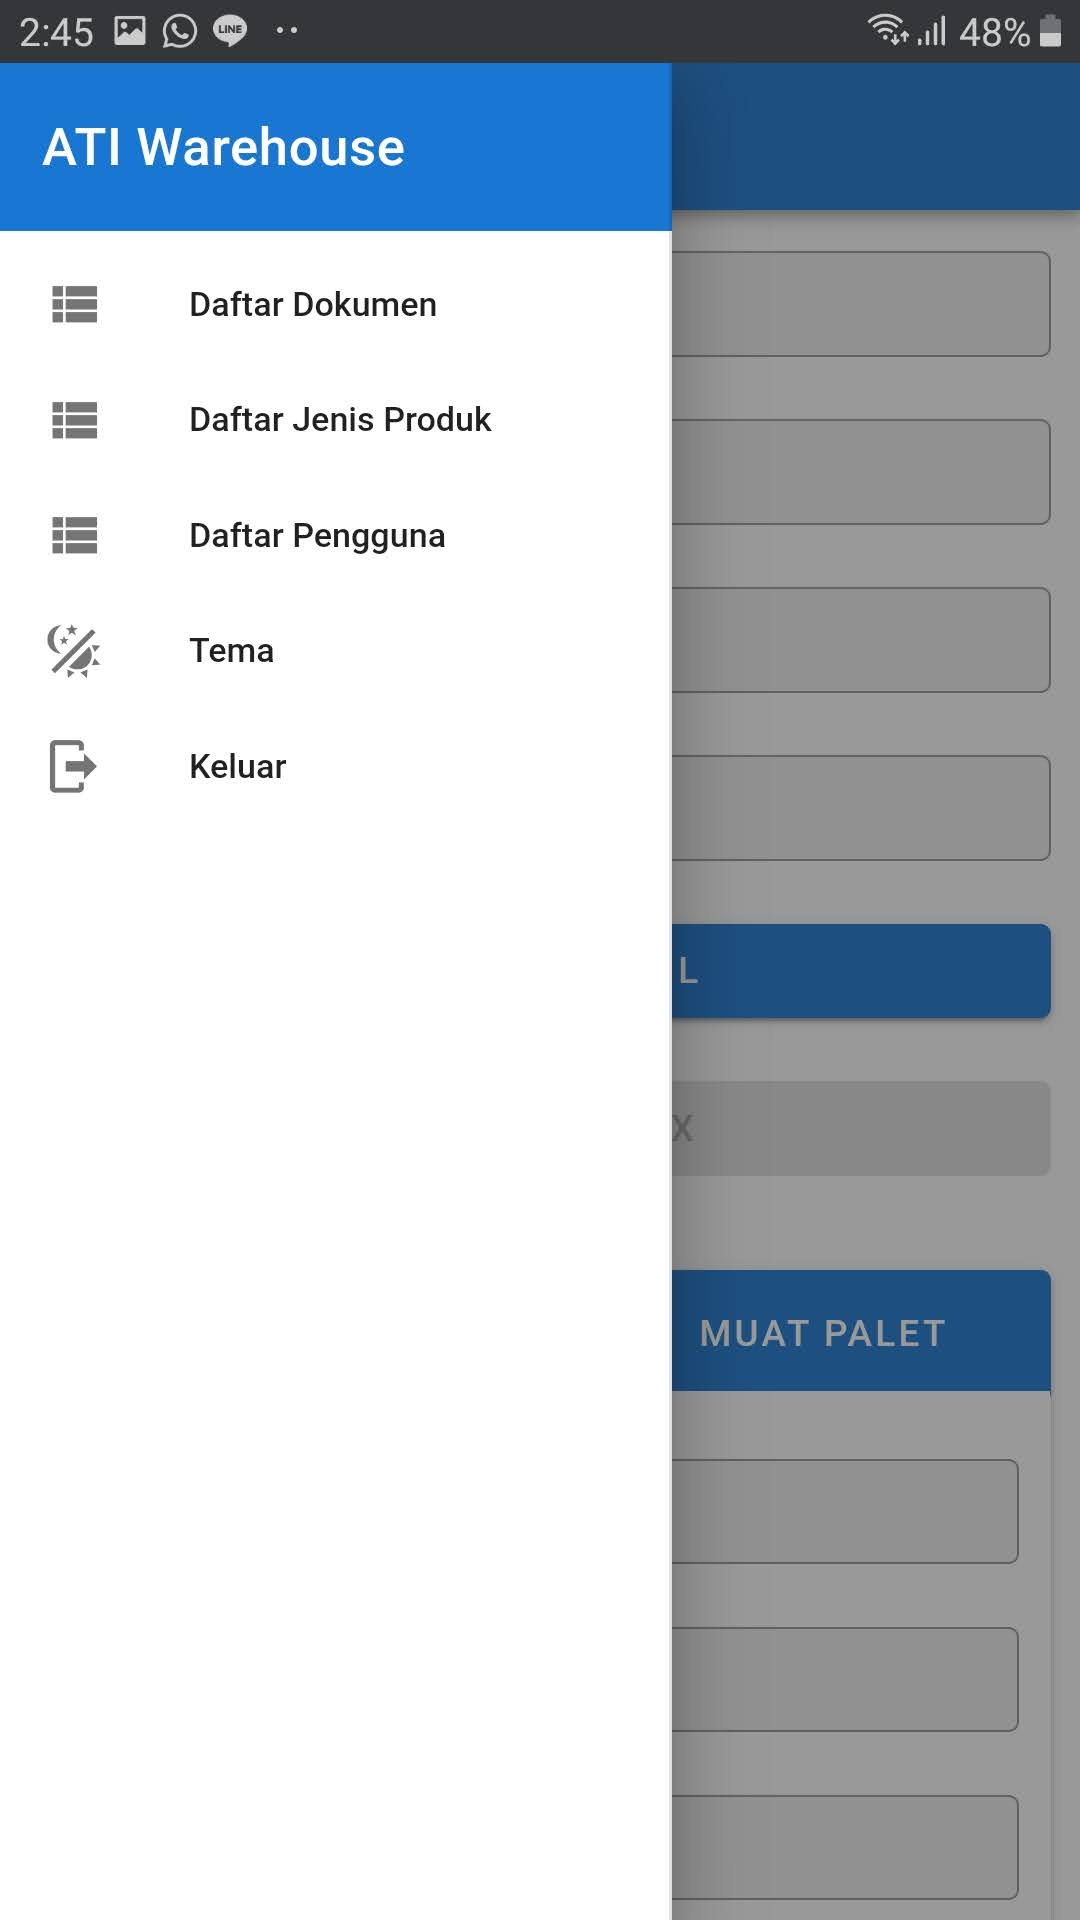
\includegraphics[width=0.45\textwidth]{gambar/tampilan-pwa-2.jpg}
  \caption{Tampilan PWA Pada Perangkat Mobile}
	\label{fig:tampilanPwa}
\end{figure}

\subsection{Menguji Pengunduhan Data Dalam Bentuk \emph{Spreadsheet}}
\vspace{1ex}

\lipsum[4]
\vspace{0.5ex}
  \cleardoublepage

  % Bab 6 kesimpulan dan saran
	% Ubah kalimat sesuai dengan judul dari bab ini
\chapter{KESIMPULAN DAN SARAN}
\vspace{4ex}

% Pengaturan ukuran indentasi
\setlength{\parindent}{7ex}

% Ubah konten-konten berikut sesuai dengan yang ingin diisi pada bab ini

\section{Kesimpulan}
\vspace{1ex}

Kesimpulan yang kami peroleh dari hasil kerja praktik ini, antara lain:
\vspace{0.5ex}

\begin{enumerate}[nolistsep]

  \item Penggunaan database yang bersifat digital dapat digunakan untuk menggantikan sistem administrasi loading barang sebelumnya yang berbasis kertas.
  \vspace{0.5ex}

  \item Data administrasi yang ditaruh di server dapat lebih mudah untuk diakses, ditambah, diubah, dan dihapus dibandingkan dengan data yang hanya berbasis kertas.
  \vspace{0.5ex}

  \item \emph{Progressive Web Apps} dapat digunakan untuk mengubah website menjadi aplikasi sehingga sistem yang dibuat bisa dengan mudah diakses pada perangkat mobile terutama jika dibutuhkan mobilitas dan kemudahan untuk melakukan pencatatan di lapangan.
  \vspace{0.5ex}

  \item Data administrasi yang ada pada server dapat diunduh dalam bentuk \emph{spreadsheet} yang bisa dicetak sehingga mempermudah pelaporan data administrasi yang masih membutuhkan bentuk kertas.
  \vspace{0.5ex}

\end{enumerate}
\vspace{0.5ex}

\section{Saran}
\vspace{1ex}

Penulis menyadari pentingnya keberadaan sistem baru yang telah dibuat ini, namun penulis menemukan beberapa hal yang kami rasa perlu untuk diperbaiki dan ditingkatkan, antara lain:
\vspace{0.5ex}

\begin{enumerate}[nolistsep]

  \item Perlunya mekanisme keamanan yang lebih baik serta backup pada data yang ada agar data yang berada di server tidak dengan mudah disalahgunakan oleh pihak yang tidak bertanggung jawab.
  \vspace{0.5ex}

  \newpage

  \item Perlunya mekanisme penyimpanan dan pengolahan data yang lebih baik agar data yang disimpan tidak memakan banyak ruang serta bisa diakses dengan lebih cepat dan optimal.
  \vspace{0.5ex}

  \item Kedepannya disarankan agar PWA yang ada bisa juga digunakan secara offline, sehingga tanpa adanya akses ke server, sistem masih bisa digunakan untuk sementara sampai akses ke server tersebut telah diperoleh kembali.
  \vspace{0.5ex}

\end{enumerate}
\vspace{0.5ex}

  \cleardoublepage

  % Daftar pustaka
  \renewcommand\bibname{DAFTAR PUSTAKA}
  \addcontentsline{toc}{chapter}{\bibname}
  \titlespacing*{\chapter}{0pt}{0ex}{5ex}
  \appendix
  \bibliographystyle{apalike}
  \bibliography{pustaka/pustaka.bib}
  \cleardoublepage

\end{document}